\chapter[Fundamentação Teórica]{Fundamentação Teórica}

O processo de gaseificação de uma biomassa para geração de energia elétrica pode ser visto na Figura \ref{fluxograma}. Ele é basicamente dividido em três principais partes: a preparação da biomassa, envolvendo o pré-tratamento e secagem da mesma, sua gaseificação, envolvendo o processo dentro do gaseificador e a limpeza dos gases de saída e a geração de eletricidade para o consumidor final \cite{chaves2016}.

\begin{figure}[!htb]
	\centering
	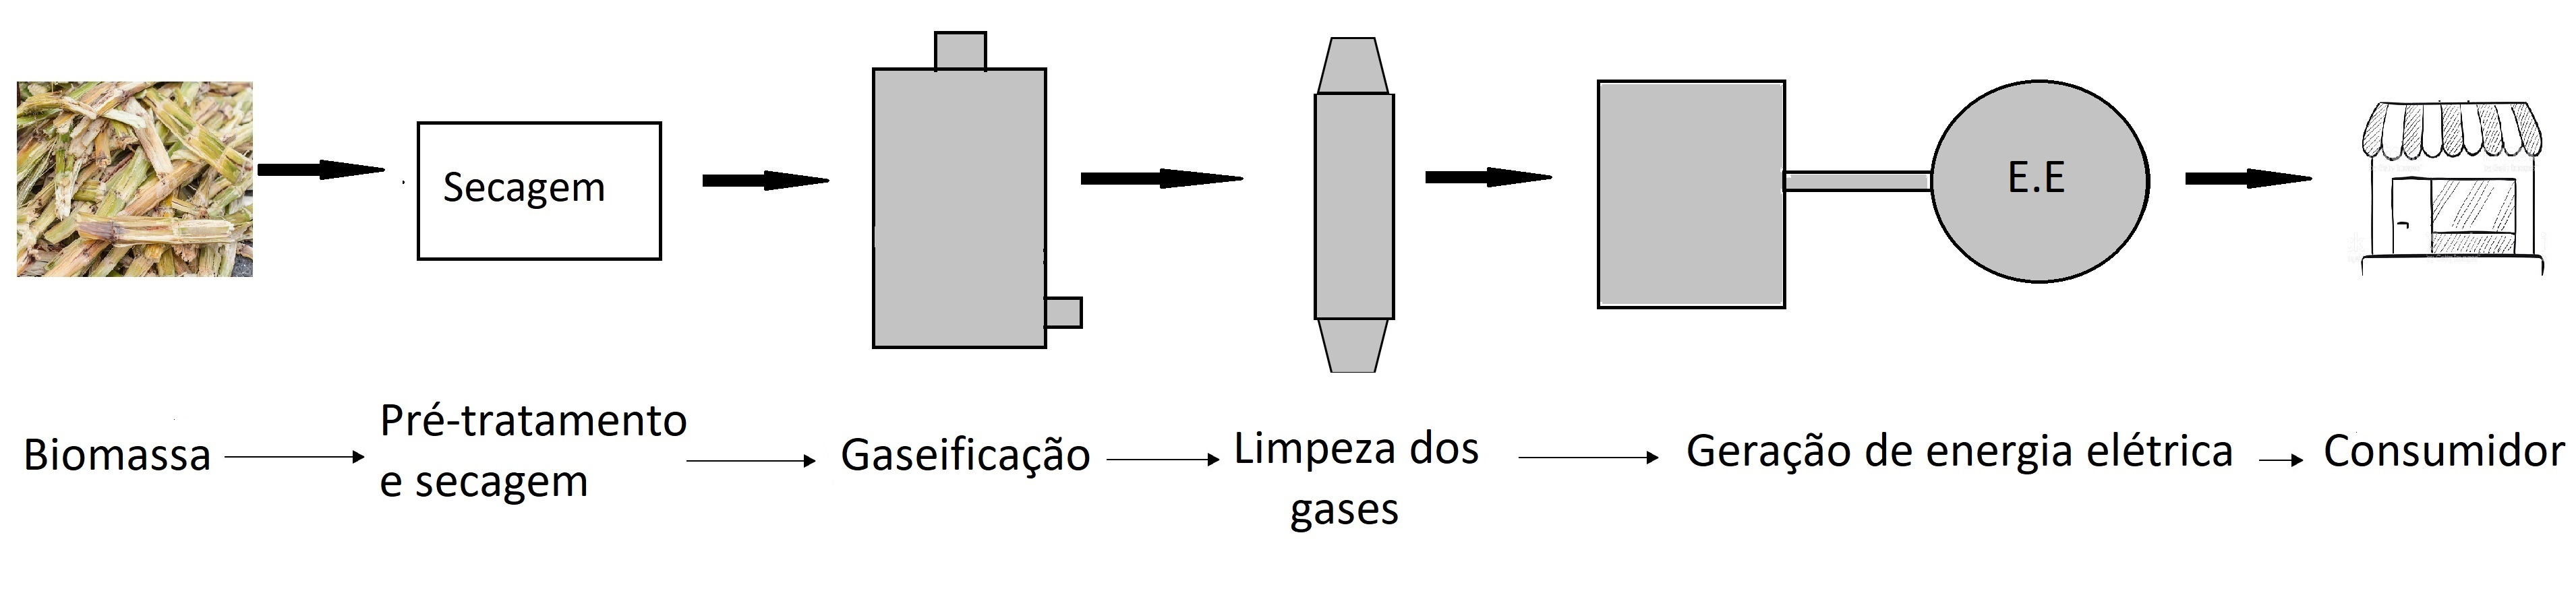
\includegraphics[width = 16cm]{fluxograma_2}
	\caption{Geração de energia elétrica por sistema de gaseificação a biomassa. (Fonte: autoria própria)}
	\label{fluxograma}
\end{figure}


\section{Biomassa}

Biomassa é definida como qualquer material orgânico derivado de organismos vivos, plantas e animais, recentemente mortos, excluindo assim os materiais fósseis. É considerada uma fonte de energia sustentável e renovável por ser formada de uma interação constante de dióxido de carbono, ar, água, solo e luz do sol \cite{basu2010}.

Ela pode ser obtida de vegetais lenhosos, resíduos agrícolas, urbanos, industriais, animais e florestais. O bagaço da cana se encontra em resíduos agrícolas e resíduos industriais, pois é um resíduo tanto das atividades agrícolas brasileiras, como dos processos industriais do setor sucroalcooleiro \cite{biomassacortez}.
	
\subsection{Caracterização da Biomassa}

A empregabilidade de uma biomassa como fonte em um sistema de geração de energia pode ser avaliada pelo potencial energético que a mesma contém, e para determinação de tal potencial, é necessário que se conheçam as propriedades químicas e térmicas da biomassa empregada, por meio das análises elementar, imediata e do seu poder calorífico.

\subsubsection{Análise imediata}

Com a análise imediata, obtém-se os valores percentuais de umidade (W), voláteis, carbono fixo e cinzas, baseando-se nas normas ASTM D 3172 a 3175, iniciando pela determinação do teor de umidade com a secagem da amostra em estufa a temperaturas entre 101$^{\circ}$C e 110$^{\circ}$C. As demais composições são determinadas elevando-se a temperatura a 750$^{\circ}$C para as cinzas e 950$^{\circ}$C para os voláteis, a diferença de peso registrada é o carbono fixo \cite{sanchez2010}.

\subsubsection{Análise elementar}

Com a análise elementar, obtém-se os valores percentuais dos elementos que compõem a amostra, que são, prinipalmente, carbono (C), hidrogênio (H), oxigênio (O), mas também nitrogênio (N) e enxofre (S) em alguns casos, determinados com base na norma ASTM D-3.176. Esta análise é importante para a determinação do volume de ar necessário para a combustão e o poder calorífico do combustível \cite{biomassacortez}

\subsubsection{Poder Calorífico}

O poder calorífico é definido como a quantidade de energia por unidade de massa liberada durante a combustão de um combustível e pode ser designado em poder calorífico superior (PCS) e poder calorífico inferior (PCI). A diferença entre os dois é a energia requerida para vaporização da água presente no combustível. O PCS pode ser determinado experimentalmente com bomba calorimétrica baseado na norma ASTM D2015 ou analiticamente utilzando a fórmula empírica de Mendeleev (equação \ref{eq:mendeleev_equation}). O PCI é dado pela diferença entre o PCS e a umidade do combustível, segundo a equação \ref{eq:pci_equation}.

\begin{equation} \label{eq:mendeleev_equation}
PCS = 4,187 [81C + 300H - 26(O - S)] kJ/kg
\end{equation}

\begin{equation} \label{eq:pci_equation}
PCI = PCS - 25,12(W + 9H)] kJ/kg
\end{equation}

A Tabela \ref{tabela_caracterizacao} mostra os resultados da caracterização do bagaço de cana baseado em vários autores em revisão da literatura feita por \cite{lenco2010}.

\begin{table}[h]
	\centering
	\caption{Caracterização do bagaço de cana segundo \cite{lenco2010}.}
	\begin{tabular}{|c|c|c|c|c|}
		\hline
		\multicolumn{2}{|c|} {\textbf{Análise Elementar}} & \multicolumn{2}{|c|} {\textbf{Análise Imediata}}  & \textbf{Poder Calorífico}\\
		\hline
		C & 45,65\% &              &        &  \\
		H &  5,98\% & Carbono fixo & 11,2\% &  \\
		O & 45,61\% & Voláteis     & 85,6\% &  18,8 MJ/kg\\
		N &  0,26\% & Cinzas       &  3,2\% &  \\	
		S &  0,08\% &              &        &  \\
		\hline		
	\end{tabular}
	\label{tabela_caracterizacao}
\end{table}	


\section{Gaseificação}

Gaseificação é um processo termoquímico que converte um combustível sólido ou líquido em um gás através de oxidação parcial a temperaturas elevadas. A tecnologia consiste em suprir a reação com quantidades restringidas de oxidante, que pode ser oxigênio puro, ar atmosférico ou vapor d’água, produzindo gás de síntese (ou syngas), que é composto, basicamente, por hidrogênio e monóxido de carbono \cite{biomassacortez}.

O gás de síntese, resultado da reação de gaseificação, pode ser aplicado na produção de combustíveis líquidos e na geração de energia mecânica e elétrica \cite{biomassacortez}. Seu poder calorífico é baseado, dentre outros fatores, no agente oxidante utilizado, como pode ser visto na Tabela \ref{tabela_agente_oxidante}.

\begin{table}[h]
	\centering
	\caption{Poder calorífico do syngas baseado no agente oxidante \cite{basu2010}}
	\begin{tabular}{|c|c|}
		\hline
		\textbf{Agente Oxidante} & \textbf{Poder Calorífico (MJ/Nm\textsuperscript{3})} \\
		\hline
		Ar & 4 - 7 \\
		Vapor d'água & 10 - 18 \\
		Oxigênio puro & 12 - 28 \\
		\hline
	\end{tabular}
	\label{tabela_agente_oxidante}
\end{table}	
		
Esses valores têm significativa influência nas aplicações do syngas. O vapor e o oxigênio, que têm um poder calorífico médio, são melhor utilizados na produção de combustíveis, já para a geração de energia elétrica através de motores e turbinas, pode-se utilizar um oxidante com baixo poder calorífico, como o ar \cite{bridgwater2003}.

\subsection{Gaseificador}

Os gaseificadores são os equipamentos onde ocorre a gaseificação da biomassa, o processo ocorre em quatro zonas principais: secagem, pirólise, combustão e redução, esta ordem depende do tipo de gaseificador utilizado. Eles são classificados pela direção do movimento da biomassa e do agente oxidante, e podem ser divididos em três grupos: leito fixo, subdivididos em contracorrente (updraft), concorrente (downdraft) e fluxo cruzado (crossdraft), leito fluidizado e leito arrastado \cite{higman2007}.
 
Os gaseificadores de leito fixo são os de mais simples construção, de maior empregabilidade e são aplicados em sistemas de pequena escala, enquanto os de leito fluidizado e leito arrastado são para média e alta escala, respectivamente \cite{basu2010}. 

\subsubsection{Leito fixo}

Nos gaseificadores contracorrente (\textbf{updraft}), a biomassa desce pela ação da gravidade enquanto o agente oxidante segue o fluxo contrário. Possuem eficiência térmica elevada, uma vez que o agente oxidante vem por baixo passando primeiro pela zona de combustão, onde está com mais elevada temperatura, pré-aquecendo a carga de combustível em seu fluxo ascendente. Porém, o syngas apresenta alto teor de alcatrão, que não passa por craqueamento na zona de combustão, o que pode causar incrustações e danos a equipamentos  mecânicos e a tubulações, inviabilizando sua aplicação para produção de energia mecânica e elétrica sem um eficiente processo de limpeza do gás \cite{sanchez2010}. São, portanto, mais adequados à aplicação para fornecimento de calor, como fornos e caldeiras. Também são ideais para biomassas com elevada umidade e concentração de cinzas \cite{basu2010}.

Nos gaseificadores concorrentes (\textbf{downdraft}), o agente oxidante segue o mesmo fluxo da biomassa e é introduzido uniformemente na zona de combustão, região de alta temperatura, onde o alcatrão passa por craqueamento, resultando em um gás de síntese com significativo menor teor de alcatrão, tornando-o mais adequado para aplicações na geração de energia mecânica e elétrica. Porém, ao seguir para a zona de redução, o gás adquire maiores quantidades de cinza e fuligem \cite{sanchez2010}. 

Nos gaseificadores de fluxo cruzado (\textbf{crossdraft}), o ar é injetado diretamente no centro da zona de combustão, onde, no mesmo patamar, o syngas é retirado a uma velocidade muito rápida e temperaturas extremamente elevadas. São adequados à aplicação na geração de energia mecânica e elétrica por possuir rápida resposta à variação de carga, porém, não se adequam muito ao uso da biomassa por possuir alta sensibilidade à umidade \cite{sanchez2010}.

Um exemplo de cada tipo dos gaseificadores de leito fixo pode ser visto na Figura \ref{gaseificadores_principais}

\begin{figure}[!htb]
	\centering
	\subfloat[a]{
		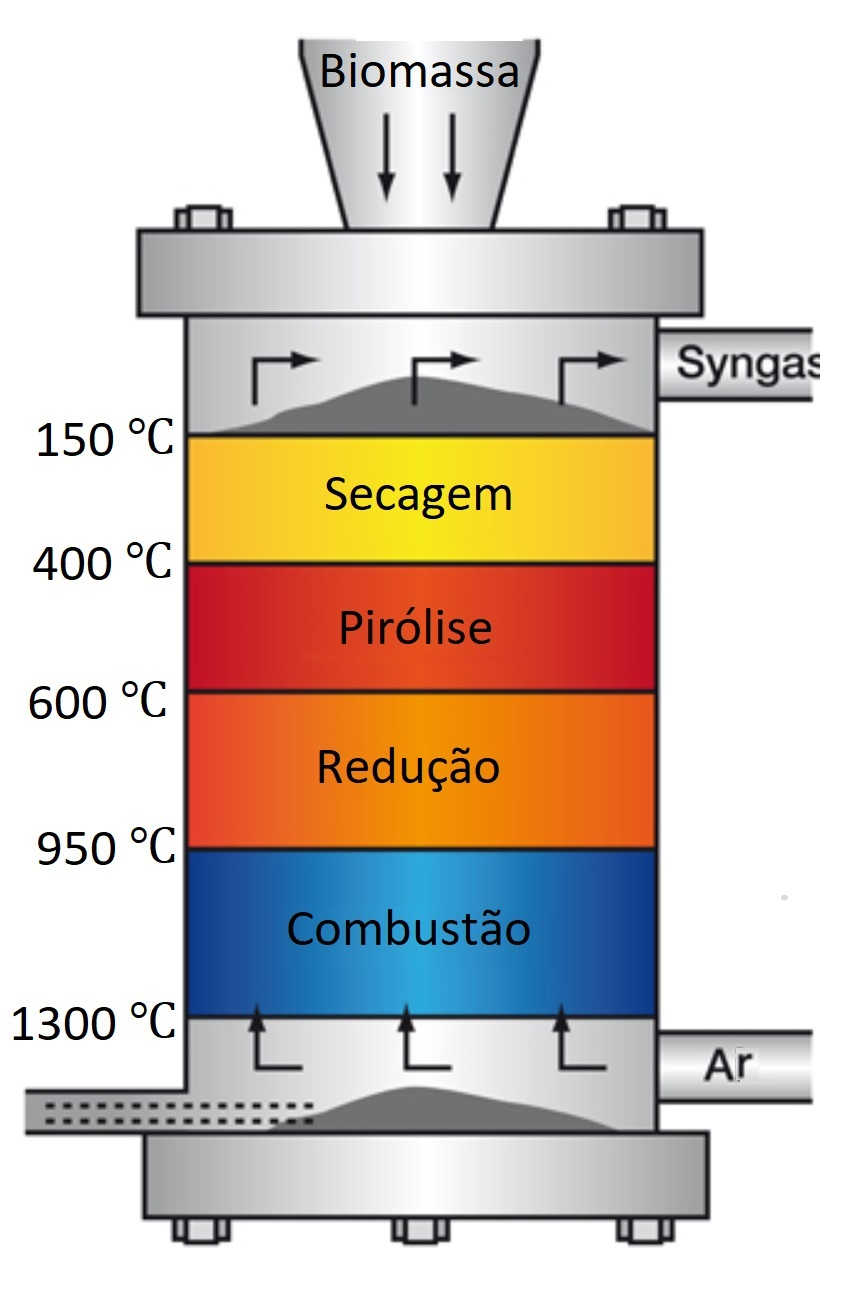
\includegraphics[width=4.2cm]{updraft_gasifier}
		\label{figdroopy}
	}
	\quad %espaco separador
	\subfloat[b]{
		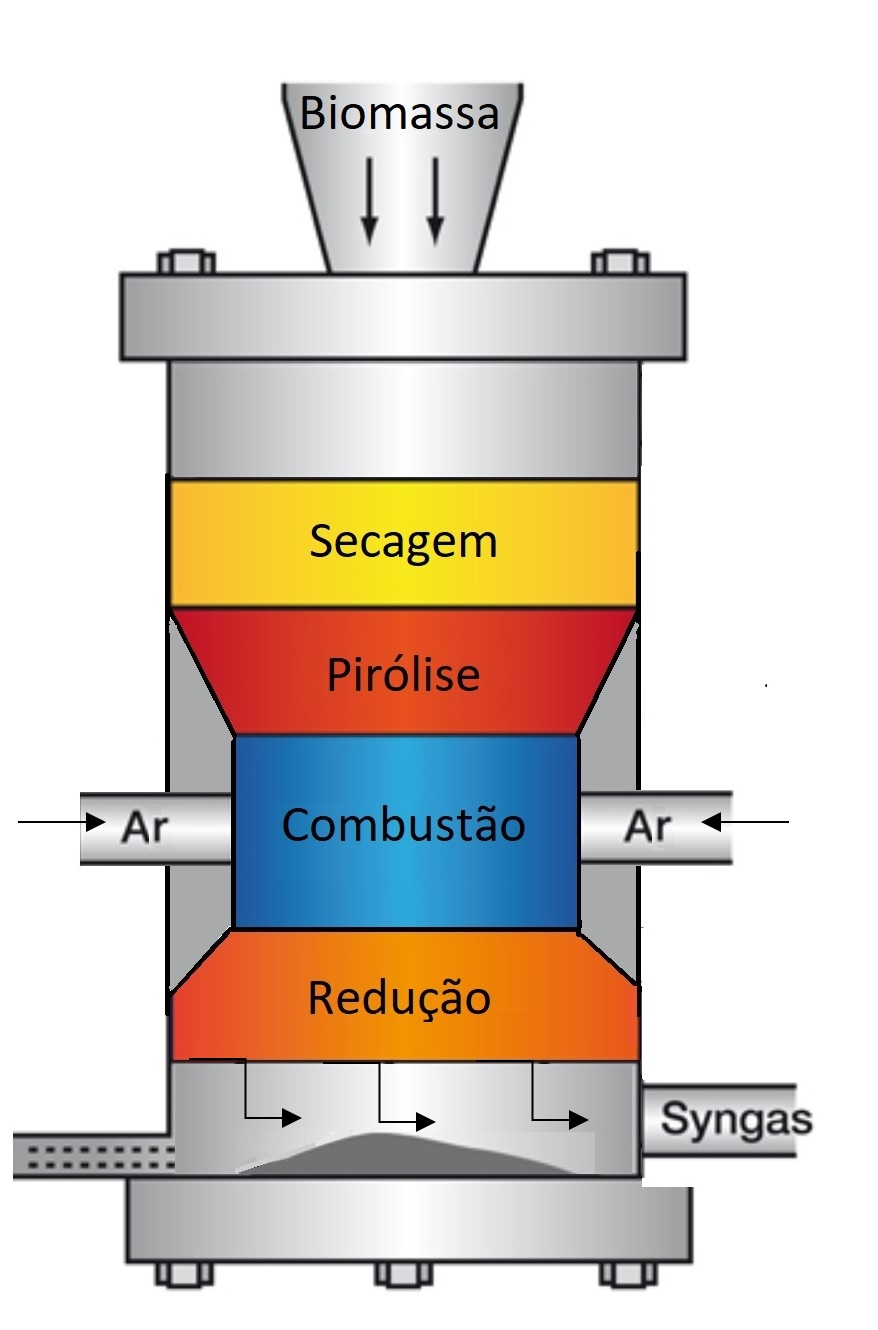
\includegraphics[width=4.2cm]{downdraft_gasifier}
		\label{figsnoop}
	}
	\subfloat[c]{
	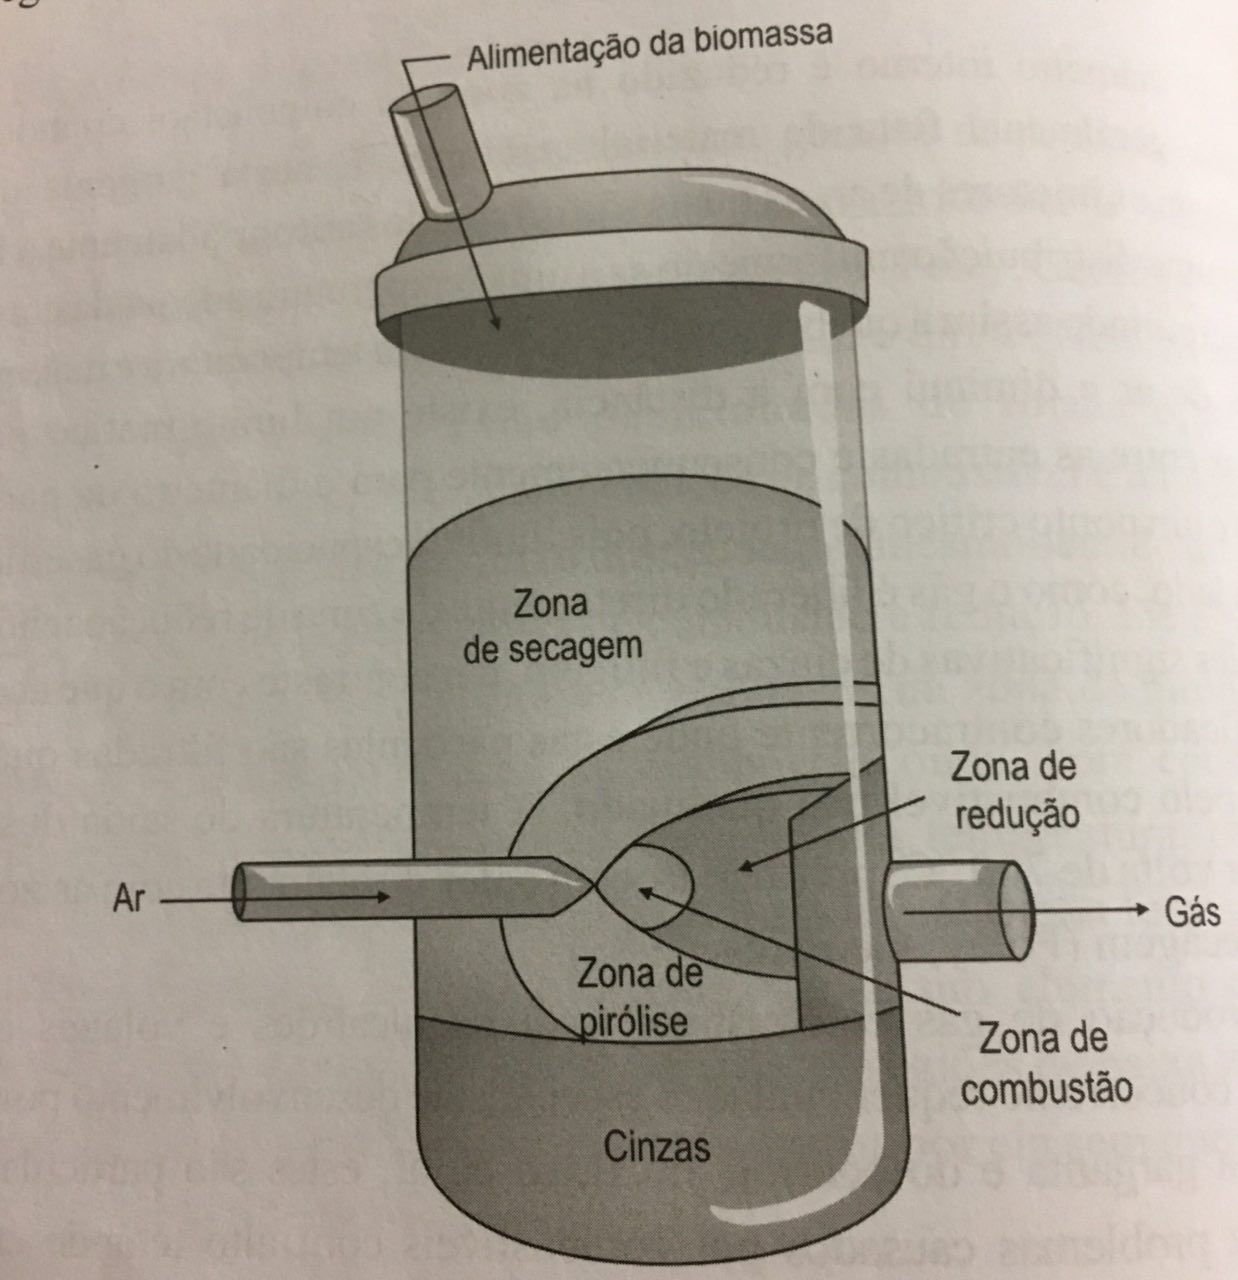
\includegraphics[width=4.5cm]{crossdraft_gasifier}
}
	\caption{Gaseificadores de Leito Fixo. [a] Gaseificador Updraft. [b] Gaseificador Downdraft. [c] Gaseificador Crossdraft \cite{mandl2009} modificado}
	\label{gaseificadores_principais}
\end{figure}


\subsubsection{Leito Fluidizado e Leito Arrastado}

Nos gaseificadores de leito fluidizado, a biomassa é introduzida em toda a extensão do gaseificador com um material inerte suportados por uma placa distribuidora, o agente oxidante sobe pelo gaseificador de forma ascendente reagindo com a mistura \cite{sanchez2010} e com velocidade suficiente para fazê-la levitar e se espalhar pela grelha até atingir o topo onde a velocidade reduz e as partículas recirculam pela grelha causando alta transferência de massa e calor entre as partículas de combustível e o agente oxidante \cite{reed1988}. 

Nos gaseificadores de leito arrastado, a biomassa e o agente oxidante seguem o mesmo fluxo dentro do gaseificador em poucos segundos. A biomassa é introduzida com um diâmetro igual ou inferior a 100 $\mu$m para que possa ser transportada pelo gás \cite{higman2007}.

Exemplos de ambos gaseificadores podem ser vistos na Figura \ref{gaseificadores_outros}

\begin{figure}[!htb]
	\centering
	\subfloat[a]{
		\includegraphics[width=5.5cm]{fluidized_bed}
	}
	\quad %espaco separador
	\subfloat[b]{
		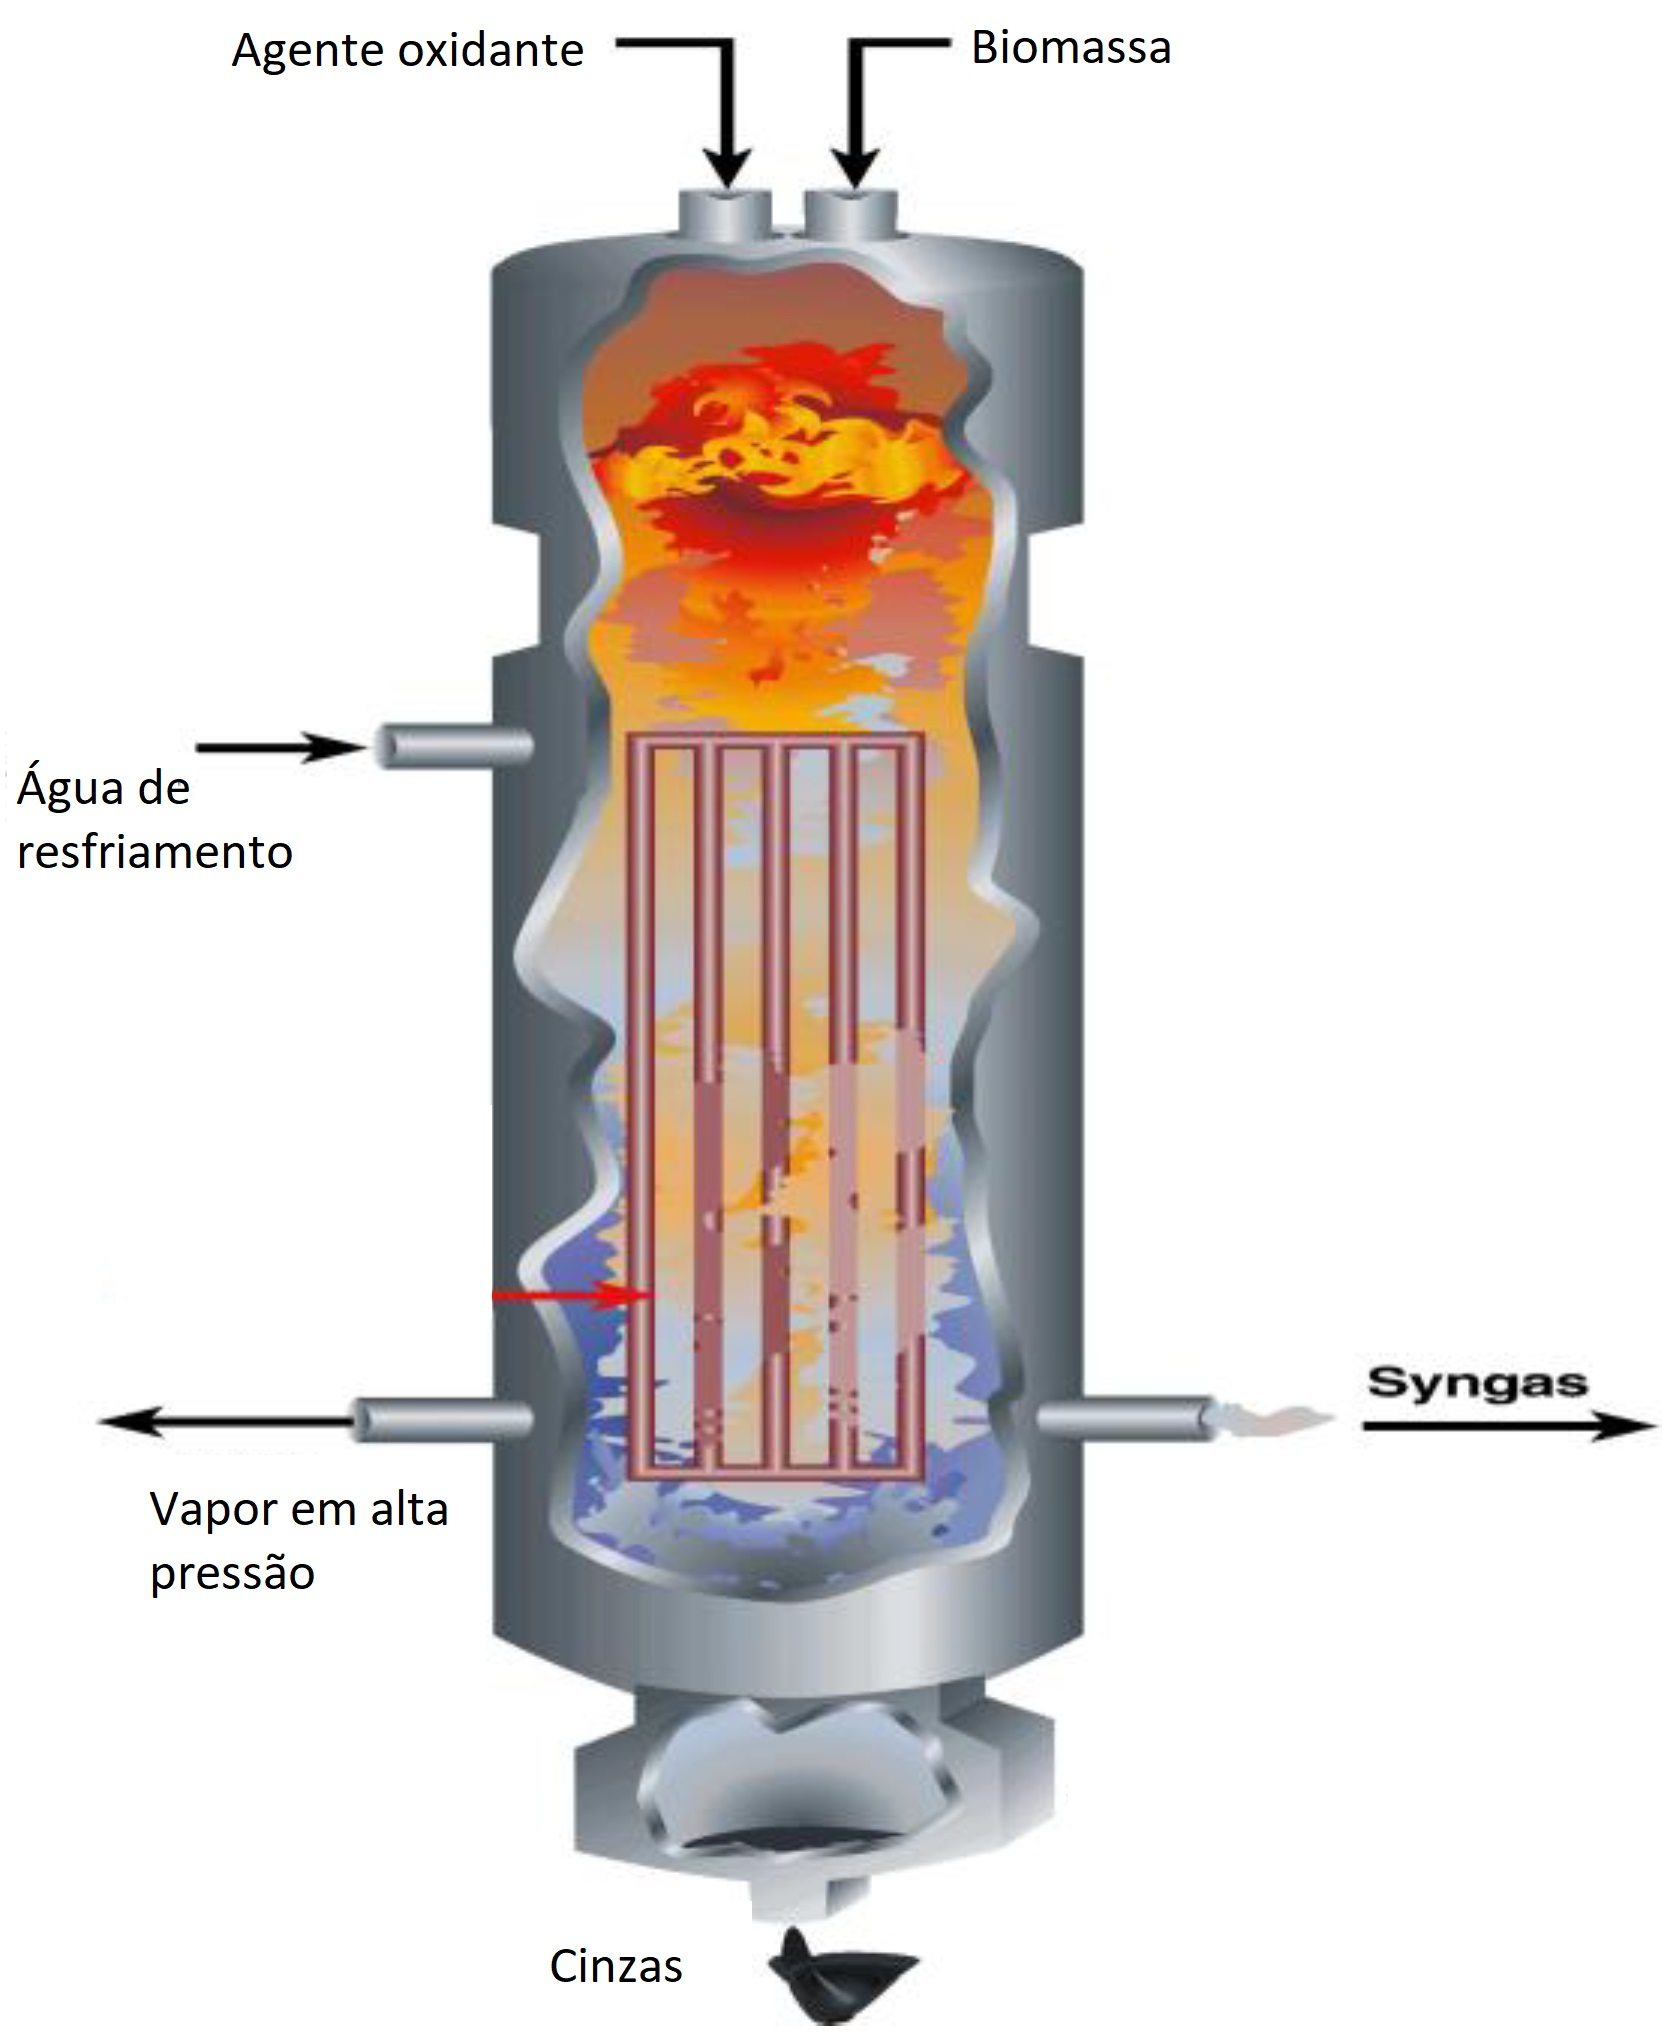
\includegraphics[width=5cm]{entrained_flow}
	}
	\caption{[a] Gaseificador de Leito Fluidizado \cite{khan2012}(modificado). [b] Gaseificador de Leito Arrastado \cite{wang2013}(modificado)}
	\label{gaseificadores_outros}
\end{figure}

\subsection{Processo de gaseificação em gaseificador downdraft}


O teor de umidade da biomassa é um inconveniente para o processo de gaseificação, pois necessita-se de um mínimo de 2260 kJ para vaporizar 1 kg de água presente na biomassa \cite{basu2010}. Além disso, para o bagaço de cana, quanto maior for o teor dessa umidade, menor é o seu poder calorífico, levando a um menor aproveitamento energético \cite{silva2008}. Dessa forma, é de suma importância que a amostra passe por um processo de secagem antes de ser introduzida no gaseificador.

A biomassa introduzida passa por outro processo de secagem em temperaturas em torno de 100-500 $^{\circ}$C, onde os valores esperados de umidade variam de 5\% a 35\%, caso ultrapassados estes valores, o poder calorífico do syngas será reduzido, resultando em queda na eficiência da conversão \cite{susastriawn2017}. 

A biomassa segue para a zona de pirólise, onde as moléculas serão quebradas em moléculas menores entre as temperaturas de 500 – 700 $^{\circ}$C, produzindo carbono, alcatrão e gases condensáveis \cite{basu2010}. 

O ar que entra na zona de combustão reage com o carbono produto da pirólise em reações exotérmicas entre 800 – 1400 $^{\circ}$C provendo calor para os demais processos do gaseificador. As reações \ref{eq:monoxido_de_carbono} e \ref{eq:dioxido_de_carbono} são referentes às reações parcial e total, respectivamente, de oxidação do carbono que ocorrem na zona de combustão.

\begin{equation} \label{eq:monoxido_de_carbono}
	C + \frac{1}{2} O_2 \rightarrow CO	\qquad \qquad	(-110,6 kJ/mol)
\end{equation}

\begin{equation} \label{eq:dioxido_de_carbono}
	C + O_2 \rightarrow CO_2	\qquad \qquad	(-393,8 kJ/mol)
\end{equation}

Na zona de redução ocorrem as principais reações de gaseificação, endotérmicas e exotérmicas, que são: a reação de Boudouard (equação \ref{eq:boudoard}), a reação heterogênea de gás-água (equação \ref{eq:gas-agua}), a reação de formação do metano (equação  \ref{eq:metano}) e as reações homogêneas de gás-gás, todas listadas abaixo (equações \ref{eq:gas-gas_1} e \ref{eq:gas-gas_2}).

\begin{equation} \label{eq:boudoard}
C + CO_2 \rightarrow 2CO	\qquad \qquad	(172,6 kJ/mol)
\end{equation}

\begin{equation} \label{eq:gas-agua}
C + H_2O \rightarrow CO + H_2 	\qquad \qquad	(131,4 kJ/mol)
\end{equation}

\begin{equation} \label{eq:metano}
C + 2H_2 \rightarrow CH_4 	\qquad \qquad	(-74,93 kJ/mol)
\end{equation}

\begin{equation} \label{eq:gas-gas_1}
CO + H_2O \rightarrow CO_2 + H_2	\qquad \qquad	(-41,2 kJ/mol)
\end{equation}

\begin{equation} \label{eq:gas-gas_2}
CH_4 + H_2O \rightarrow CO + 3H_2 	\qquad \qquad	(201,9 kJ/mol)
\end{equation}




\section{Sistema de limpeza do syngas}

O syngas produzido, como pode ser visto pelas equações, é composto de monóxido de carbono, dióxido de carbono, hidrogênio e metano, sua qualidade é determinada pelo processo de gaseificação adotado e pelas características físicas e químicas da biomassa \cite{chaves2016}.

Antes de ser encaminhado para o motor, o syngas deve ser previamente tratado devido à presença de alcatrão e cinzas. Para que o motor opere em condições satisfatórias, a concentração de alcatrão em um motor de combustão interna deve ser menor que 100mg/Nm\textsuperscript{3} \cite{hasler1999}. 

Há dois métodos de remoção de alcatrão para limpeza dos gases, primário e secundário. No método primário, o gaseificador é modificado para redução da formação de alcatrão no gás, por exemplo, com a adição de uma segunda injeção de ar. No método secundário, o alcatrão é removido após sair do gaseificador, através de remoção física ou catalítica. A remoção física pode ser feita por ciclones, filtros de barreira, precipitadores eletrostáticos ou lavadores com água. Necessita-se que o alcatrão seja primeiramente condensado antes do processo de separação \cite{basu2010}. Um exemplo de filtro pode ser visto na Figura \ref{filtro}.

\begin{figure}[!htb]
	\centering
	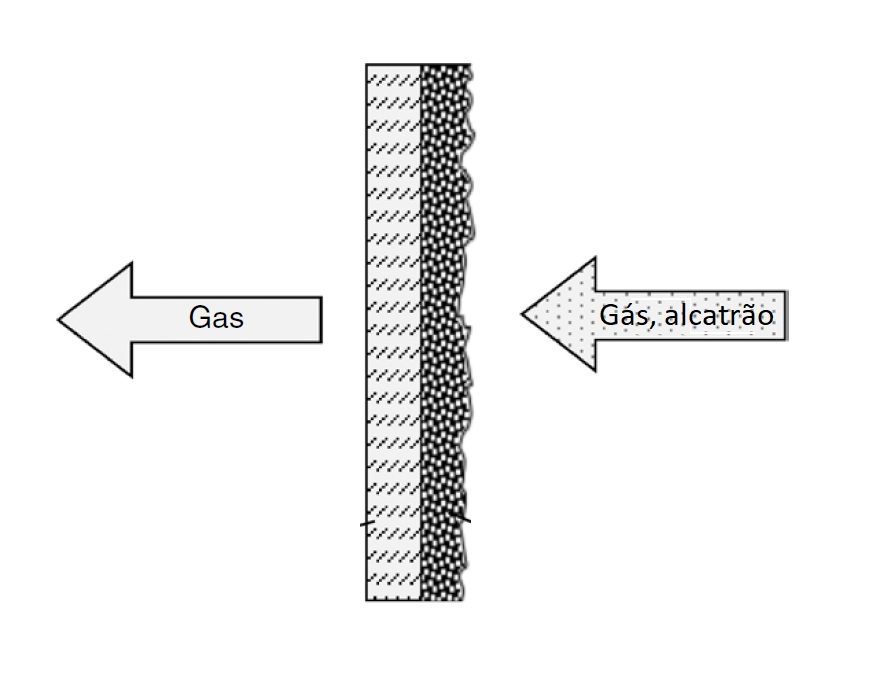
\includegraphics{filtro}
	\caption{Método de remoção de alcatrão: Filtro de barreira (\cite{basu2010})}
	\label{filtro}
\end{figure}


\section{Grupo Moto-gerador}
Após o sistema de limpeza, o syngas segue para o grupo moto-gerador, que será responsável pela geração de energia elétrica. As tecnologias utilizadas para geração de energia elétrica a partir do syngas produzido no gaseificador podem ser motor de combustão interna, motor stirling, microturbinas e células a combustíveis, sendo que o motor de combustão interna apresenta maior maturidade tecnológica e comercial \cite{lora2006} e, comparado aos demais, menor custo por kw \cite{chaves2016}.


\section{Geração Distribuída}

O conceito de geração distribuída não é consensual dentre os autores da literatura. Em seu artigo, \cite{ackermann2001} faz uma revisão da literatura quanto à definição de GD segundo diferentes aspectos, tais como: localização, potência instalada, tecnologia, modo de operação e impacto ambiental e define geração distribuída como geração de energia elétrica próxima ao consumidor dentro da rede de distribuição.

A prinicpal vantagem relacionada ao emprego da geração distribuída é a redução de perdas associadas à transmissão da energia elétrica, que não é necessária pois é gerada no próprio local de consumo. As demais vantagens podem ser destacadas com a qualidade e confiabilidade da energia gerada, pois o sistema não aceita variação de tensão ou frequência, atendimento conforme a demanda e diminuição da dependência do parque gerador \cite{barbosa2013}. 

No Brasil, o setor de geração distribuída é regulamentado pela Agência Nacional de Energia Elétrica (ANEEL), que, em sua Resolução Normativa Nº 482, de 17 de abril de 2012 estabeleceu as condições gerais para o acesso de microgeração e minigeração distribuída aos sistemas de distribuição de energia elétrica e o sistema de compensação de energia elétrica. Segundo as definições da resolução, microgeração distribuída é uma central geradora com potência instalada menor ou igual a 75kW e para minigeração distribuída é entre 75kW > x < 5MW. A compensação de energia elétrica é definida como \textit{"sistema no qual a energia ativa injetada por unidade consumidora com microgeração ou minigeração distribuída é cedida, por meio de empréstimo gratuito, à distribuidora local e posteriormente compensada com o consumo de energia elétrica ativa"}.

\section{Estado da Arte}
Estudos e experimentos mostraram sistemas de gaseificação para geração de energia elétrica em pequena escala com resultados satisfatórios. 

\cite{figueiredo2012} gaseificou lenha de eucalipto em um sistema de gaseificador downdraft e motor de combustão interna acoplado a um gerador de 50kVA com o objetivo de avaliar a viabilidade de se aplicar o sistema em localidades distantes. A produção de syngas conseguiu suprir a demanda máxima do gerador (26,4kW), consumindo aproximadamente 49,6 kg/h de biomassa. 

\cite{chaves2016} utilizou um sistema com gaseificador downdraft e motor com ignição por faísca acoplado a um gerador alimentado por lascas de madeira, que apresentou uma eficiência no processo de gaseificação de 60-70\%, decaindo para 4,5-17\% de eficiência na geração elétrica, devido ao poder calorífico da biomassa e à eficiência térmica do motor.

\cite{yoon2012} utilizou casca de arroz em um gaseificador downdraft de bancada com um motor à gas natural modificado para usar o syngas, alimentando 40-60 kg/h de biomassa e ar como agente oxidante, conseguindo gerar 10kW.

\cite{dasappa2011} realizou experimento operacional com sistema de gaseificação de 100kWe conectado à rede, composto por reator downdraft, sistema de resfriamento e limpeza dos gases e grupo moto-gerador. O sistema operou por 1000h, consumindo 107kg/h de biomassa, gerando uma energia total de 80,6MWh com eficiência de aproximadamente 18\%.






